\chapter{Data}
\label{ch:data}

% TODO get rid of LiDAR!
For our formulation of shape completion,\ie Problem \ref{problem}, we require two sources
of data: the shape set $\mathcal{Y}$ to learn the shape prior and the observations $\mathcal{X}$
in order to learn maximum likelihood or an extended variational auto-encoder.
For research purposes,
however, we created three synthetic datasets also including the ground truth
shapes $\mathcal{Y}^*$ corresponding to $\mathcal{X}$ for evaluation: a
dataset of rectangles in 2D, a dataset of cuboids in 3D and
a dataset of cars from ShapeNet \cite{ChangFunkhouserGuibasSavarese:2015}
in 3D. Besides providing both observations $\mathcal{X}$ and ground
truth $\mathcal{Y}^*$, these datasets also
reflect the progress made in the course of the thesis. For brevity,
we will only present experiments in 3D; details on the
2D dataset can be found in Appendix~\ref{ch:appendix-data}.
Furthermore, we present experiments on the point clouds provided
by KITTI \cite{GeigerLenzUrtasun:2012,GeigerLenzStillerUrtasun:2013}.
In this case, we use car models from ShapeNet as shape set~$\mathcal{Y}$
and the provided 3D bounding boxes to extract the corresponding observations~$\mathcal{X}$.
However, on KITTI, we are not able to quantitatively
evaluate the proposed approaches due to missing ground truth shapes $\mathcal{Y}^*$.
In the following, we introduce our process of generating synthetic 3D datasets,
\ie the 3D cuboids dataset and the ShapeNet dataset, and extracting the observations
from KITTI.

\section{3D Example and ShapeNet}
\label{sec:data-3d}

Our 3D datasets consist of arbitrarily scaled and rotated
cuboids or cars; the cuboids are generated on-the-fly, while we use the
car models from ShapeNet.
The models are provided in the form of triangular meshes such that we
need to consider the following processing steps: voxelization and filling
of the shapes; rendering, backprojecting and voxelization of the observations;
and finally post-processing to compute signed distance functions. 
This will provide us with both observations and ground truth shapes; to
learn the shape prior, and simulate the realistic case,
we then voxelize and fill a separate set of shapes. The overall
process is also illustrated in Figure \ref{fig:data-3d-process} and discussed in
detail in the following.

\begin{figure}
  \centering
  \vspace{-1cm}
  \begin{tikzpicture}
    \node[
      %rectangle,draw=black
    ] at (-1, 0) {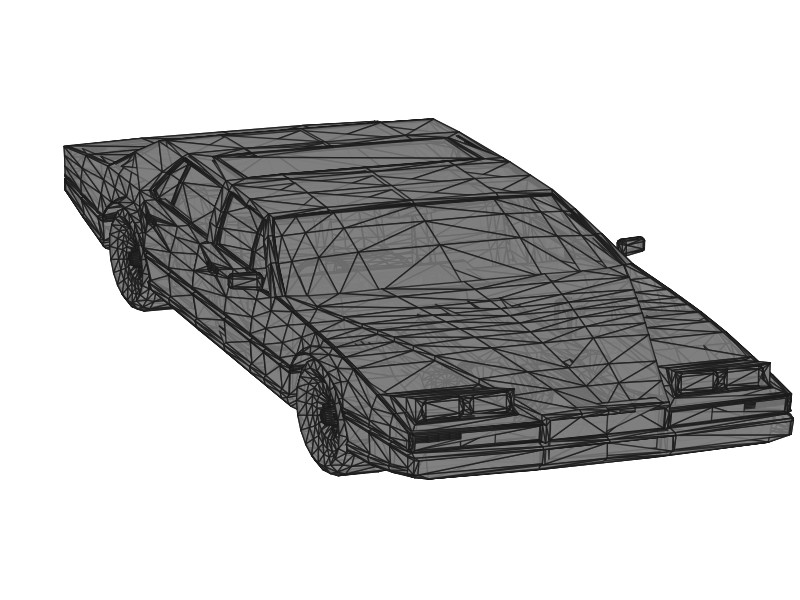
\includegraphics[height=2.25cm]{data/shapenet/dd84236f0ef27765a134736201a79843}};
    
    \node at (4, 0) {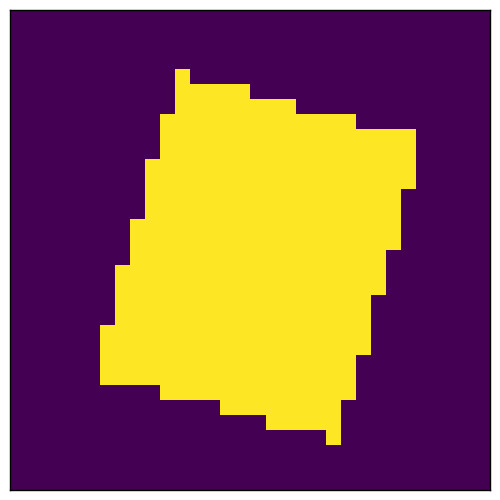
\includegraphics[height=3cm]{data/shapenet/0}};
    %\node at (4, -2.5) {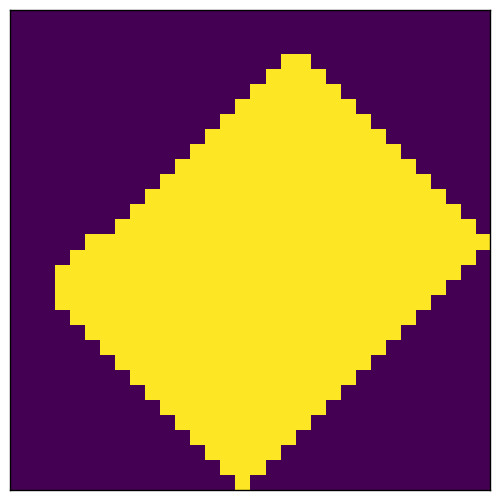
\includegraphics[height=3cm]{data/shapenet/1}};
    %\node[rectangle,draw=black,minimum width=3.75cm,minimum height=5cm] at (4,-1.25) {};
    
    \node at(9, 0) {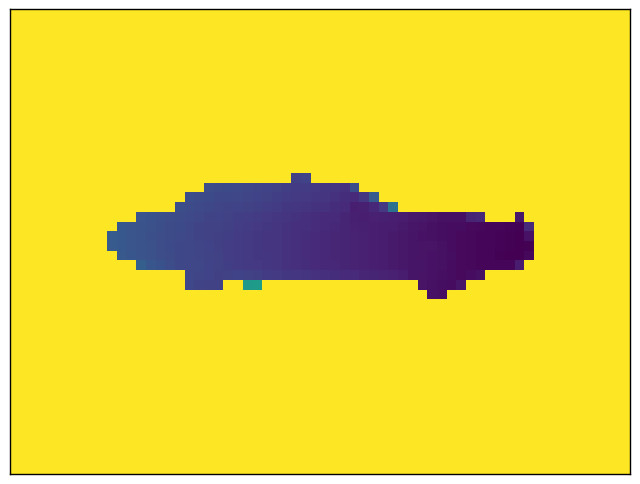
\includegraphics[height=2.5cm]{data/shapenet/0_depth}};
    %\node at(9, -2.5cm) {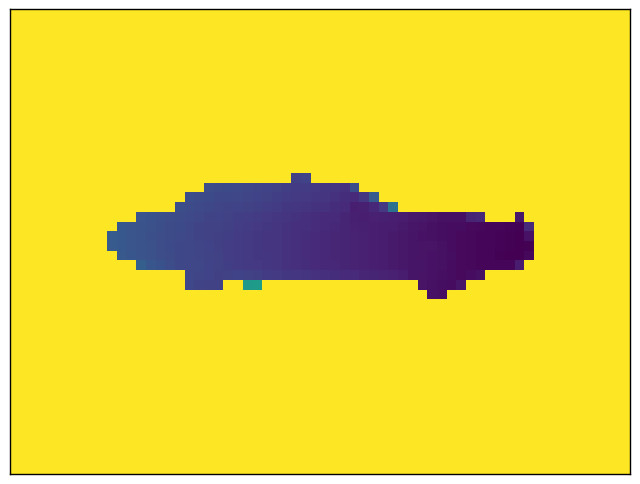
\includegraphics[height=2.5cm]{data/shapenet/0_depth}};
    %\node[rectangle,draw=black,minimum width=3.35cm,minimum height=5cm] at (9,-1.25) {};
    
    \draw[->] (1, 0) -- (2, 0);
    \node at (1.5,0.3) {(a)};
    
    \draw[->] (6, 0) -- (7, 0);
    \node at (6.5,0.3) {(b)};
    
    \node at (4, -3.5) {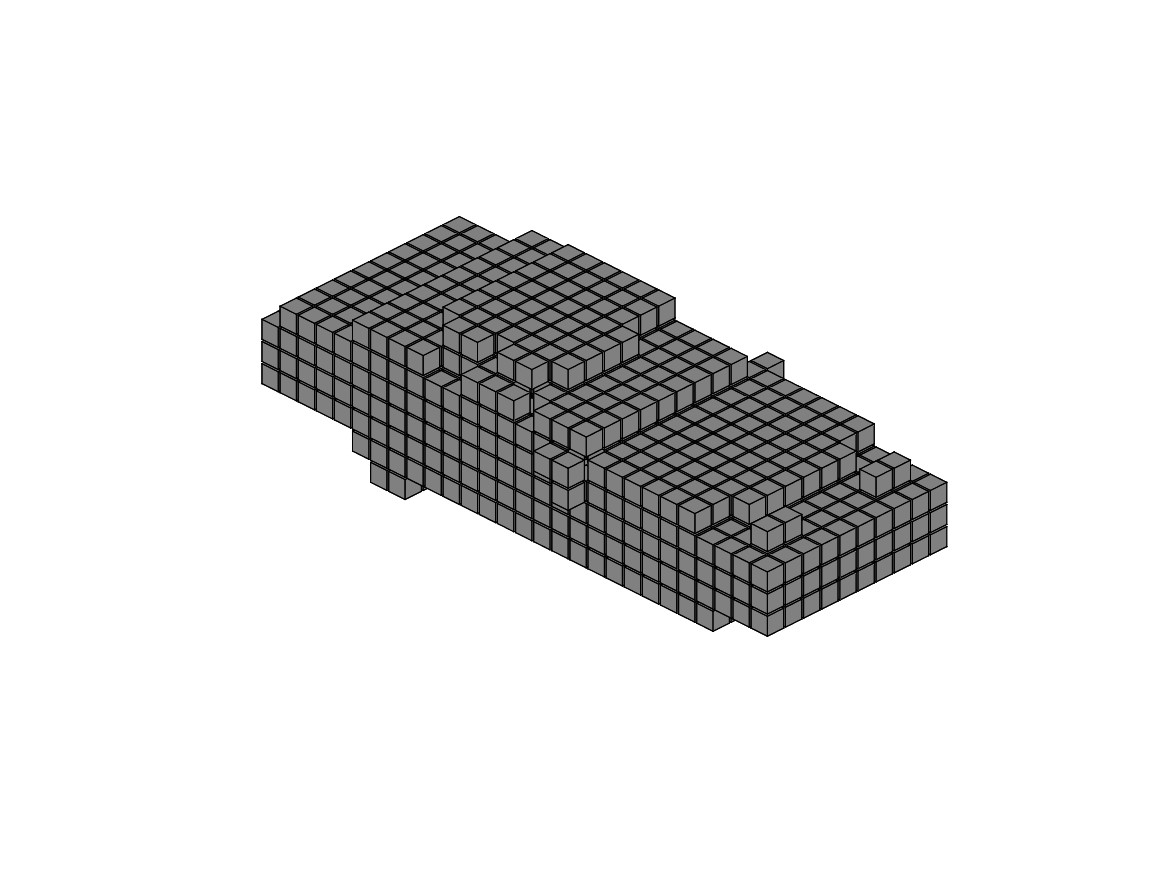
\includegraphics[height=2.5cm,trim={2cm 1cm 2cm 1cm},clip]{data/shapenet/1_output}};
    
    \node at (9, -3.5) {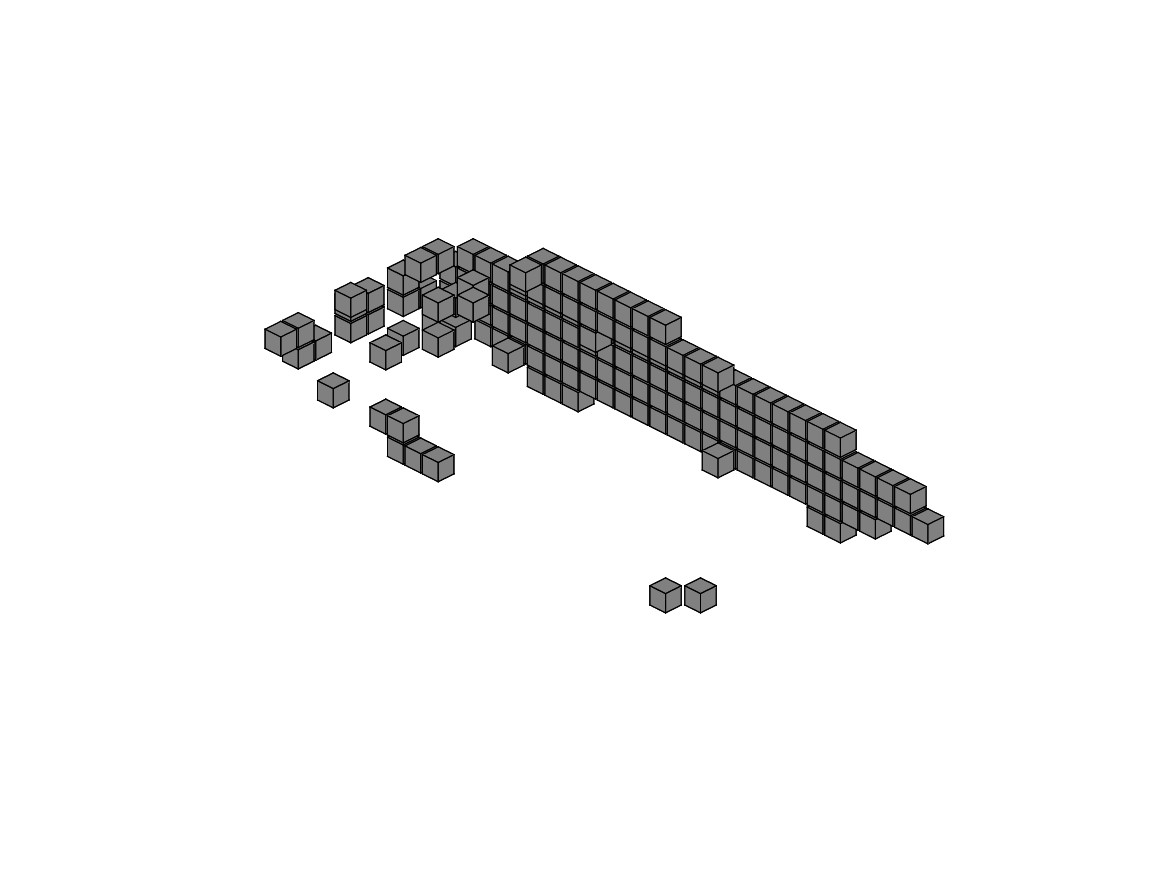
\includegraphics[height=2.5cm,trim={2cm 1cm 2cm 1cm},clip]{data/shapenet/1_input}};
    %\node at (9, -5.5) {\includegraphics[height=2.5cm]{data/shapenet/0_real_space}};
    
    \draw[->] (4,-1.5) -- (4, -2.5);
    \node at (4.4,-2) {(c)};
    
    \draw[->] (9,-1.5) -- (9, -2.5);
    \node at (9.4,-2) {(d)};
    
    \node at (-2,-4.7) {(e)};
    \draw[-,dashed] (-3,-5) -- (11,-5);
    
    \node[anchor=east] at (0.75,-6) {\footnotesize Voxelized Shape};
    \node[anchor=east] at (0.75,-7) {\footnotesize Filled Shape};

    \node[anchor=east] at (0.75,-8) {\footnotesize Voxelized Points};
    \node[anchor=east] at (0.75,-9) {\footnotesize Voxelized Free Space};

  \node[anchor=east] at (0.75,-10) {\footnotesize \begin{tabular}{r@{}}Distance Function\\for Points\end{tabular}};
    \node[anchor=east] at (0.75,-11) {\footnotesize \begin{tabular}{r@{}}Distance Function\\for Free Space\end{tabular}};

    \node[anchor=east] at (0.75,-13.25) {\footnotesize \begin{tabular}{r@{}}Signed Distance\\Function for Shape\end{tabular}};

    \node at (6,-6.5) {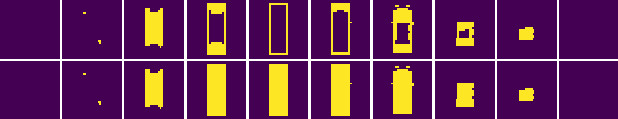
\includegraphics[width=10cm]{data/shapenet/0_output_slices}};
    \node at (6,-9.5) {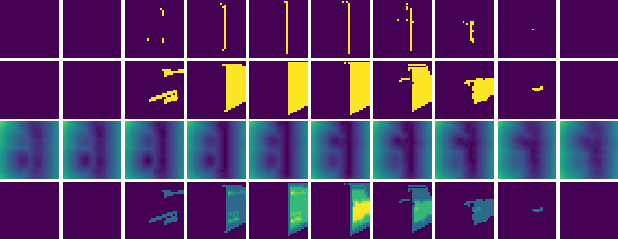
\includegraphics[width=10cm]{data/shapenet/0_sdf_slices}};
    \node at (6,-12) {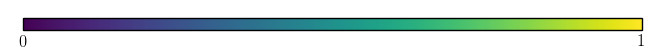
\includegraphics[width=10.8cm]{data/shapenet/colorbar}};
    \node at (6,-13.25) {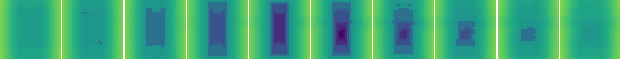
\includegraphics[width=10cm]{data/shapenet/0_sdf_output_slices}};
    \node at (6,-14.1) {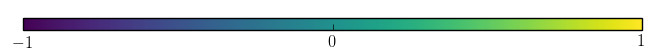
\includegraphics[width=10.8cm]{data/shapenet/sdf_colorbar}};
  \end{tikzpicture}
  % TODO short caption
  \caption{Illustration of the data generation process on an example from
  the ShapeNet dataset. The original triangular mesh is
  shown in the top left. In (a), it is first simplified using the approach outlined in
  Algorithm \ref{alg:data-hull}. The simplified mesh is rendered, (b), from
  a random viewpoint. The simplified mesh is then voxelized using triangle-box
  intersections, (c), and the rendered depth map is used to generate and voxelize
  the observations, (d). Finally, in (e), the corresponding signed distance
  functions are computed. The top two rows show the filling process of the voxelized
  mesh, the next four rows show the observed points and observed free space
  and the corresponding distance functions; the last row shows the
  signed distance function of the filled mesh. Each row shows 
  horizontal slices of the corresponding volumes, \ie heights $11 + i$ for $0 \leq i < 10$.}
  \label{fig:data-3d-process}
\end{figure}

\subsection{Mesh Pre-Processing and Voxelization}

We prefer to work with watertight meshes; for the 3D cuboids we have control
about this as we automatically generate the meshes. In the case of ShapeNet
this is problematic. In addition, ShapeNet may contain very complex models 
where we need to deal with up to $100000$ faces.
%\footnote{
%  We manually chose a subset of all car models in ShapeNet to
%  sort out models that could not automatically be scaled to $[0,1]^3$
%  or where the dominant orientation could not be automatically determined.
%}
Often, these models
contain a level of detail that we are not interested in as it will be
lost during voxelization, especially in low resolution. Therefore,
we decided to follow \cite{GueneyGeiger:2015}\footnote{
  \url{http://www.cvlibs.net/software/semi_convex_hull/}.
} and compute a so-called
semi-convex hull.

% TODO for if really bold!
\begin{algorithm}[t]
  \small
	\begin{algo}{Semi-Convex Hull}{
	\label{alg:data-hull}
	\qinput{triangular mesh $\mathcal{M}$}
	\qoutput{simplified mesh $\mathcal{M}^{(T)}$}
	}
	  draw sample points $\mathcal{P}$ from $\mathcal{M}$\\
	  compute convex hull $\mathcal{M}^{(0)} = (V^{(0)}, F^{(0)})$ of $\mathcal{M}$\\
	  remesh $\mathcal{M}^{(0)}$ using \cite{FuhrmannAckermannGoesele:2010}\\
		\qfor $t = 0$ \qto $T - 1$\\
		  \qif $\mathcal{M} \not\subseteq \Vol(V^{(t)})$\\
		    \qthen find smallest $\alpha > 0$ such that $P \subseteq \Vol((1 + \alpha)V^{(t)})$\\
		    $V^{(t)} := (1 + \alpha) V^{(t)}$\\
		    remesh $\mathcal{M}^{(t)}$ using \cite{FuhrmannAckermannGoesele:2010}\qfi\\
		  $V^{(t + 1)} = V^{(t)} - \gamma \nabla \mathcal{L}(V^{(t)})$\qrof\\
		\qreturn $\mathcal{M}^{(T)}$
	\end{algo}
	% TODO short caption
	\caption{The semi-convex hull algorithm used in \cite{GueneyGeiger:2015}
	to obtain watertight, simplified meshes. Details can be found in the text.}
\end{algorithm}

Algorithm \ref{alg:data-hull} first samples a set of points $\mathcal{P}$ from the
given mesh $\mathcal{M} = (V, F)$. Then, a convex hull is computed -- 
a standard problem in computational geometry, see
\cite{Cormen:2009} or \cite{DeBergCheongVanKreveldOvermars:2008}.
To reduce the number of initial vertices, the approach of
\cite{FuhrmannAckermannGoesele:2010} is used to remesh the
initial mesh. The remeshed convex hull, $\mathcal{M}^{(0)}$,  is then
iteratively refined by minimizing a loss
\begin{align}
  \mathcal{L}(V^{(t)}) = \sum_{v \in V^{(t)}} \min_{p \in \mathcal{P}} \|v - p\|_2^2 + \sum_{(i, j) \in E(F^{(t)})}\left(\|v_i - v_j\|_2^2 - \mu\right)
\end{align}
using gradient descent. Here, $\mu$ is the mean edge length
of the initial mesh $\mathcal{M}^{(0)}$. A problem with this formulation is
that at any iteration $t$, the mesh $\mathcal{M}^{(t)}$ might not
contain the point set $\mathcal{P}$ anymore. In this case,
the vertices are rescaled as $V^{(t)} := (1 + \alpha)V^{(t)}$ such that
$\mathcal{P} \subseteq \Vol(V^{(t)})$, \ie the point set
$\mathcal{P}$ is contained in the volume spanned by $V^{(t)}$
and the mesh $M^{(t)}$ is remeshed again. Results of simplification
are shown in Figure \ref{fig:data-simplification}.

\begin{figure}
  \centering
  \hspace*{-0.25cm}
  \begin{subfigure}[t]{0.24\textwidth}
    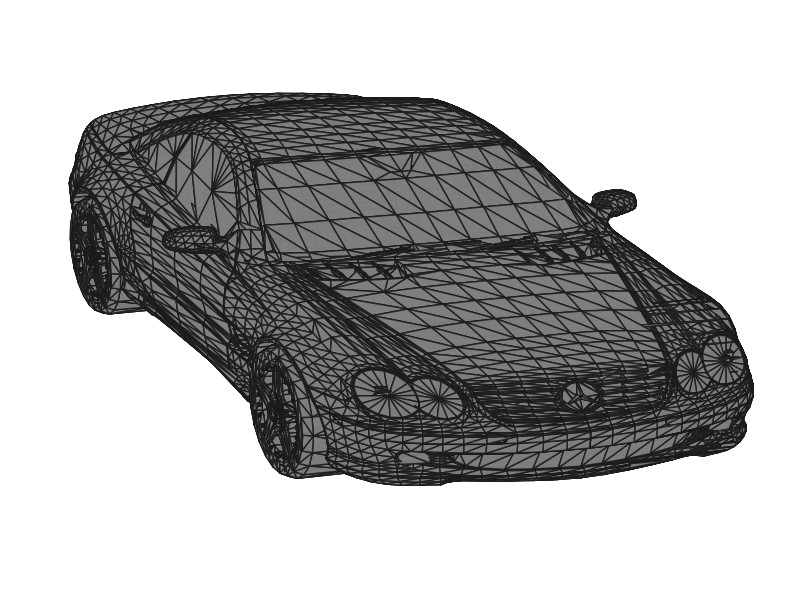
\includegraphics[height=2.5cm]{data/shapenet/simplification/119033fe083145e22f31600ac759c763}
  \end{subfigure}\hfill
  \begin{subfigure}[t]{0.24\textwidth}
    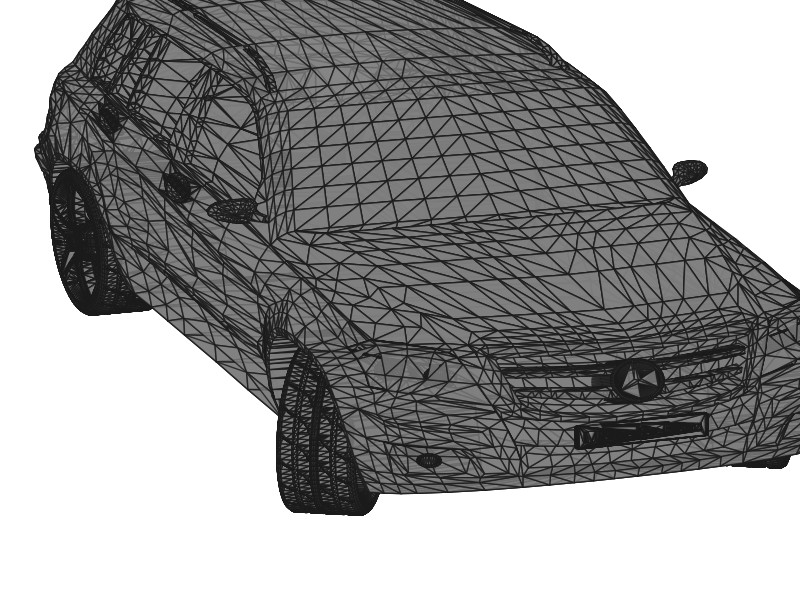
\includegraphics[height=2.5cm]{data/shapenet/simplification/109567d7d55b8fe515a520abec2f04dd}
  \end{subfigure}\hfill
  \begin{subfigure}[t]{0.24\textwidth}
    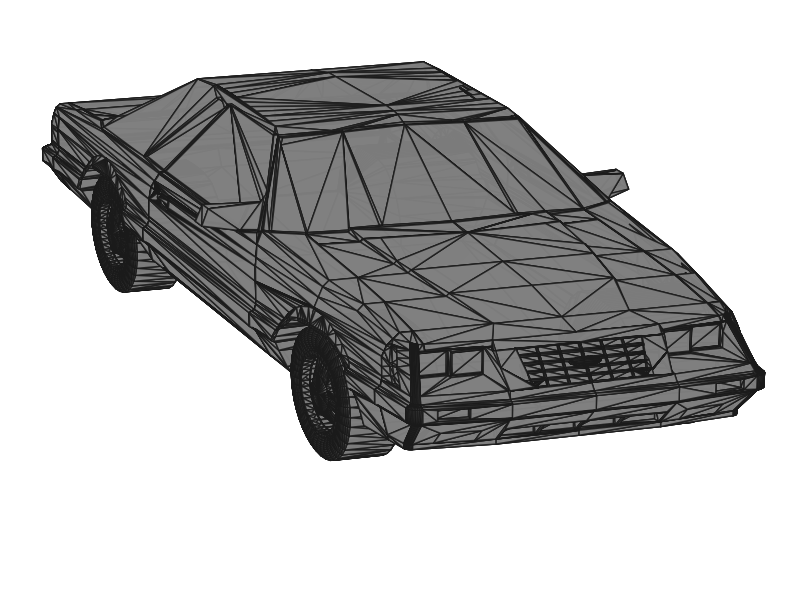
\includegraphics[height=2.5cm]{data/shapenet/simplification/1089cbe82dc0e72133d7c9e122eec9b6}
  \end{subfigure}\hfill
  \begin{subfigure}[t]{0.24\textwidth}
    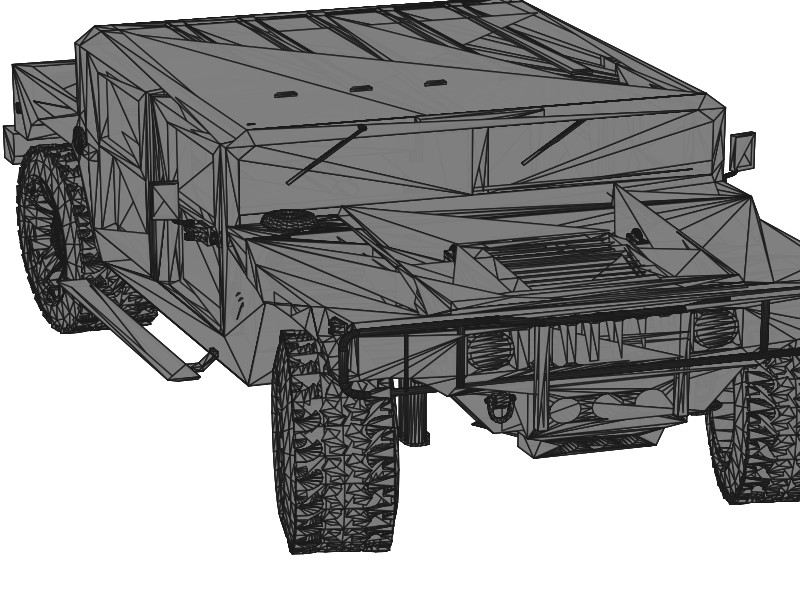
\includegraphics[height=2.5cm]{data/shapenet/simplification/100c3076c74ee1874eb766e5a46fceab}
  \end{subfigure} \\ 
  
  \begin{subfigure}[t]{0.24\textwidth}
    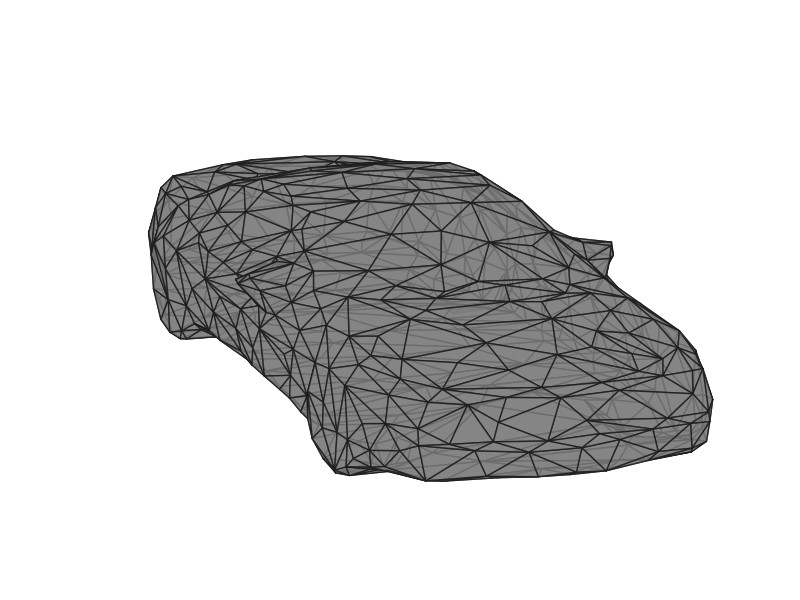
\includegraphics[height=2.7cm]{data/shapenet/simplification/0028}
  \end{subfigure}\hfill
  \begin{subfigure}[t]{0.24\textwidth}
    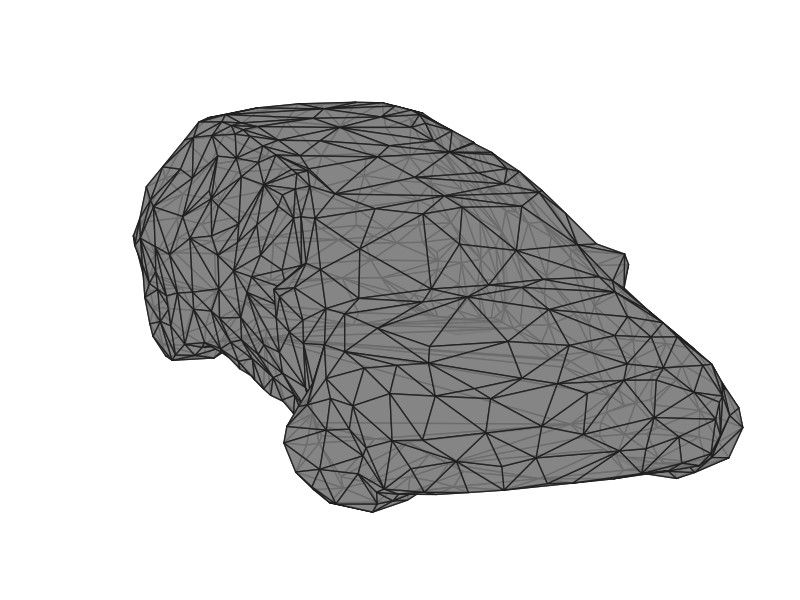
\includegraphics[height=2.7cm]{data/shapenet/simplification/0011}
  \end{subfigure}\hfill
  \begin{subfigure}[t]{0.24\textwidth}
    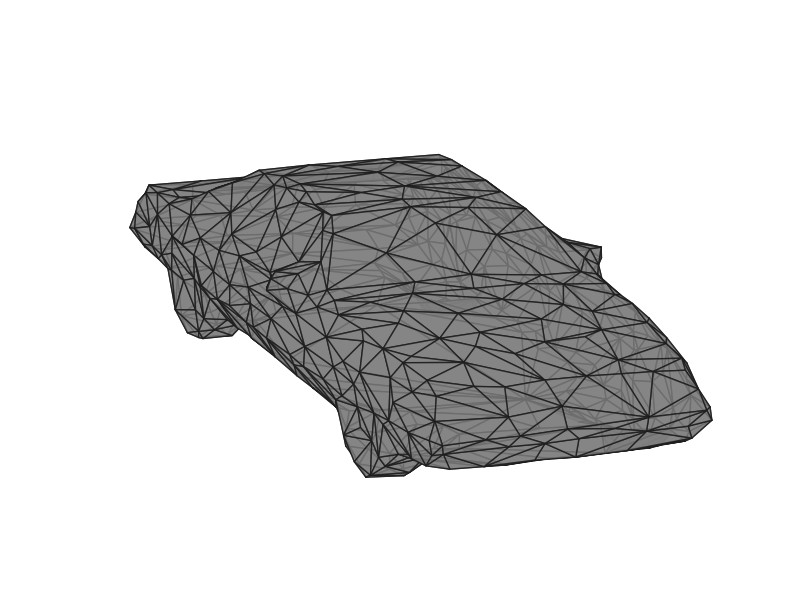
\includegraphics[height=2.7cm]{data/shapenet/simplification/0010}
  \end{subfigure}\hfill
  \begin{subfigure}[t]{0.24\textwidth}
    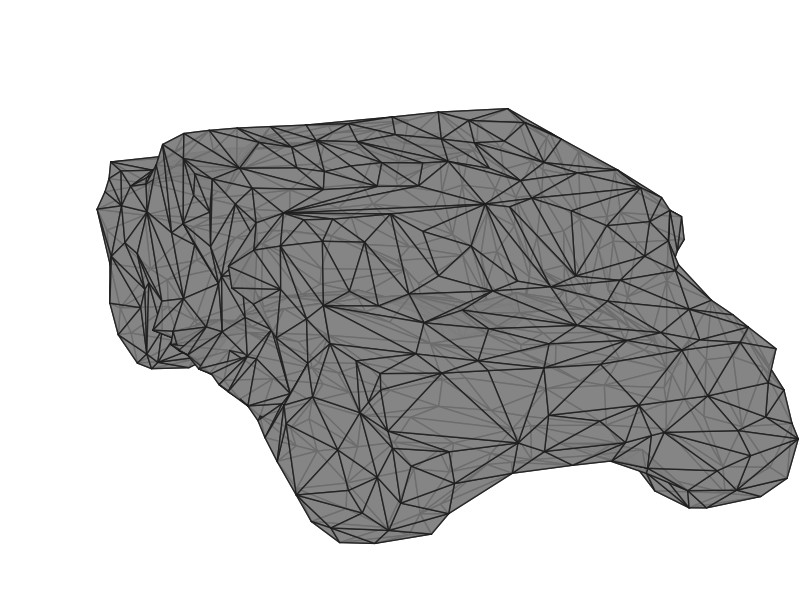
\includegraphics[height=2.7cm]{data/shapenet/simplification/0002}
  \end{subfigure}
  
  % TODO short caption
  \caption{Illustration of the employed mesh simplification approach, \ie
  Algorithm \ref{alg:data-hull}, on manually selected examples from ShapeNet.
  These show the variety available in the dataset.}
  \label{fig:data-simplification}
\end{figure}

After obtaining simple, watertight meshes, voxelization is performed using
triangle-voxel intersection tests as \eg proposed in\cite{AkenineMoeller:2001}\footnote{
  We also use the corresponding code from \url{http://fileadmin.cs.lth.se/cs/Personal/Tomas_Akenine-Moller/code/}.
}. In practice we scale, translate and pad all models to $[0,1]^3$,
which is then subdivided into $H \times W \times D$ axis-aligned voxels.
For the car models, care has to be taken to avoid skewing the models during
scaling, translating and padding. Note that all axes are scaled equally and we may
consider slight random rotation, translation and scaling for data augmentation.

\subsection{Mesh Filling}
\label{sec:data-3d-filling}

% TODO appendix multi-resolution approach
In order to obtain proper occupancy grids, \ie also identify interior
voxels, we use a flood filling/connected components algorithm
\cite{Dillencourt:1992}\cite[Section~3.3]{Szeliski:2011}.
As we work with watertight meshes, interior and exterior of the shapes
are clearly separated. For low resolutions, \eg $32^3$, this approach
works very well.

\subsection{Mesh Rendering and Observation Voxelization}

For simplicity, we use an OpenGL based MatLab renderer to obtain depth images from the pre-processed meshes.
To this end, we use the code also used in \cite{GeigerWang:2015,GueneyGeiger:2015}\footnote{
  \url{http://www.cvlibs.net/software/librender/}
}. Using the camera parameters used by OpenGL, the pixels in the depth image can
be back-projected into 3D space. By thresholding the depth value,
we know which pixels correspond to points on the mesh surface. By controlling
the depth image resolution as well as focal length, we indirectly control
the sparsity of the obtained point cloud. Using ray tracing we can additionally
derive free space. The process is described in detail in the following.

\begin{definition}
  \label{def:data-2d-camera}
  A (simplified) 2D projective camera is a tuple $(\mathcal{K}, \mathcal{R}, t)$
  where
  \begin{align}
    \mathcal{K} = \left[\begin{matrix}
      f_u & 0 & u\\
      0 & f_v & v\\
      0 & 0 & 1\\
    \end{matrix}\right]
  \end{align}
  is the intrinsic camera matrix,
  $\mathcal{R} \in \mathbb{R}^{3 \times 3}$ is a rotation matrix and
  $t \in \mathbb{R}^3$ a translation vector. Here, $f_u$ and $f_v$ are focal lengths
  along horizontal and vertical direction, respectively,
  and $(u, v)^T$ defines the principal point of the 2D image -- implicitly
  also defining its resolution, $2u \times 2v$, assuming that $(u,v)^T$ represents the
  center pixel.
\end{definition}

% TODO precise dimensions, also for 2D
The overall projection matrix of a camera $(\mathcal{K}, \mathcal{R}, t)$ is given by
$\mathcal{P} = \mathcal{K} \left[\begin{matrix}\mathcal{R} & t\end{matrix}\right] \in \mathbb{R}^{3 \times 4}$
and defines the projection of point $p = (p_1, p_2, p_3, 1)^T$ in homogeneous coordinates
to the corresponding pixel
\begin{align}
  x = \left[\begin{matrix}
    \frac{\tilde{x}_1}{\tilde{x}_3}\\
    \frac{\tilde{x}_2}{\tilde{x}_3}\\
    1
  \end{matrix}\right]\quad\text{ with }\quad \tilde{x} = \mathcal{P} p.
\end{align}
The inverse projection is defined as
its pseudo-inverse \cite[Chapter~6]{HartleyZisserman:2006}:
\begin{align}
  \mathcal{P}^+ = (\mathcal{P}^T \mathcal{P})^{-1} \mathcal{P}^T \in \mathbb{R}^{4 \times 3}
\end{align}
The ray corresponding to a pixel $x$ in homogeneous coordinates, \ie
$x = (x_1, x_2, 1)^T$, can then be obtained as
\begin{align}
  r = \left[\begin{matrix}
    \frac{\tilde{r}_1}{\tilde{r}_4}\\
    \frac{\tilde{r}_2}{\tilde{r}_4}\\
    \frac{\tilde{r}_3}{\tilde{r}_4}\\
    1
  \end{matrix}\right]
  \quad\text{ with }\quad \tilde{r} = \mathcal{P}^+ x
\end{align}
The corresponding 3D point can be derived when knowing the depth $d$ corresponding
to the ray $r$:
\begin{align}
  p = \left[\begin{matrix}
    d\cdot \frac{r_1}{r_3}\\
    d\cdot \frac{r_1}{r_3}\\
    d
  \end{matrix}\right]
\end{align}
In practice, we can also work in the camera's coordinate system such that
$\mathcal{R} = I$ and $t = 0$. As a result, the inverse projection matrix simplifies to
$\mathcal{P}^+ = \mathcal{K}^{-1}$. Then, we capture the shapes in
different rotations around the (vertical) height axis -- corresponding to
different viewpoints of the camera. After back-projection,
ray-voxel intersection tests \cite{WilliamsBarrusMorleyShirley:2005}\footnote{
  \url{http://www.cs.utah.edu/~awilliam/box/}
} can be used to determine free space voxels and occupied voxels can be determined
using point-voxel intersection tests. We rotate and translate the observations
to $[0, 1]^3$ and use the exact same subdivision into $H \times W \times D$
axis-aligned voxels as before. This way, the observations are aligned with the
corresponding ground truth shapes. To obtain free space voxels, we only consider
rays to points on the corresponding shape. We refer to the result as partial
free space as we do not consider rays corresponding to points on the background.
This is reasonable as rays from background points cannot be used reliably
on real data, \eg on KITTI.

\subsection{Noise}

To simulate real conditions, we want to inject artificial noise.  As we will see on the
KITTI dataset, correctly simulating the Velodyne sensor and the corresponding noise is
not trivial. We manually inspected many samples from the KITTI dataset and decided
to define two noise parameters, $\lambda_{\text{hit}}$ and $\theta_{\text{ignore}}$.
The former defines an exponential distribution \cite[Chapter~11]{Bishop:2006}:

\begin{definition}
  Let $\epsilon \in \mathbb{R}$, $\epsilon \geq 0$, be a random variable.
  Then $\epsilon$ is distributed according to
  an exponential distribution, \ie $\epsilon \sim \Exp(\epsilon;\lambda)$, with 
  parameter $\lambda$ if the probability density function is given by
  \begin{align}
    p(\epsilon) = \lambda \exp(-\lambda \epsilon).
  \end{align}
\end{definition}

Following inverse transform sampling \cite[Chapter~11]{Bishop:2006},
we draw samples from this distribution using $u \sim U(0,1)$ and
\begin{align}
  \epsilon = \frac{-\ln u}{\lambda}.
\end{align}
For each pixel in the depth image, we sample an error value
$\epsilon \sim \Exp(\epsilon;\lambda_{\text{hit}})$ from an
exponential distribution and add the value to the actual depth value.
This is reasonable, as $\epsilon$ will always be non-negative and $p(\epsilon)$
decreases exponentially for rising $\epsilon$.
The probability $\theta_{\text{ignore}}$ defines how likely an observation
is to be ignored. In this case, the depth value of the corresponding pixel is
set to the maximum depth.

\subsection{Discussion}

\begin{figure}
  \centering 
  \begin{subfigure}[t]{0.425\textwidth}
    \vspace{0px}
    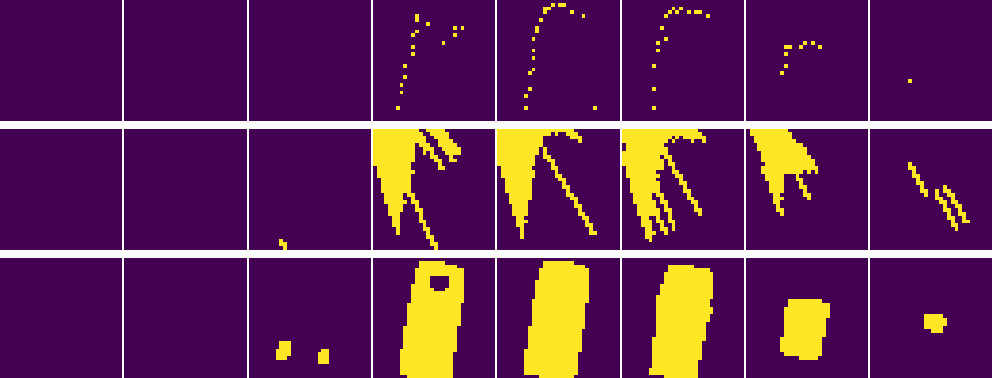
\includegraphics[width=6cm]{data/shapenet/hard/data_6_0}\\
    \hspace*{-0.25cm}\includegraphics[width=6.5cm]{data/shapenet/easy/colorbar_0}
  \end{subfigure}
  \begin{subfigure}[t]{0.2\textwidth}
    \vspace{0px}
    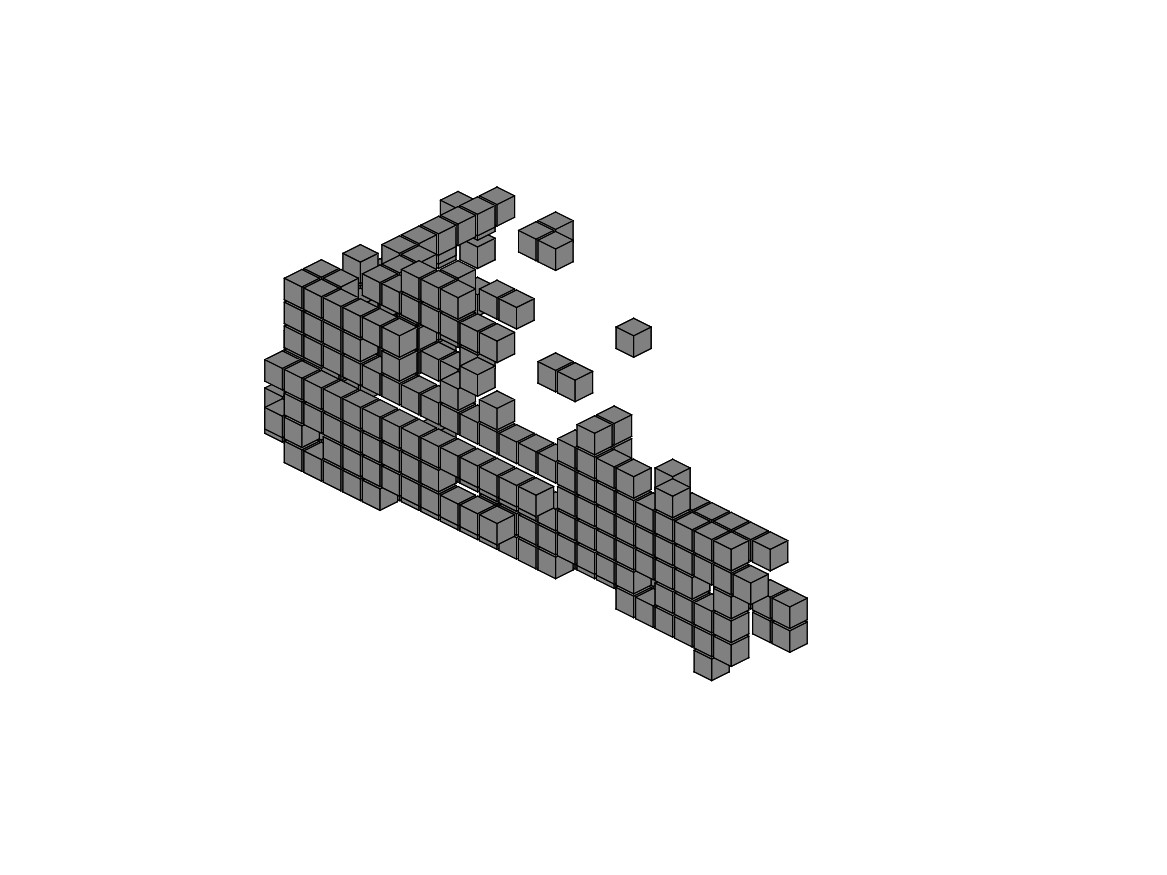
\includegraphics[width=3cm,trim={2cm 1cm 2cm 1cm},clip]{data/shapenet/hard/6_input_45}
  \end{subfigure}
  \begin{subfigure}[t]{0.2\textwidth}
    \vspace{0px}
    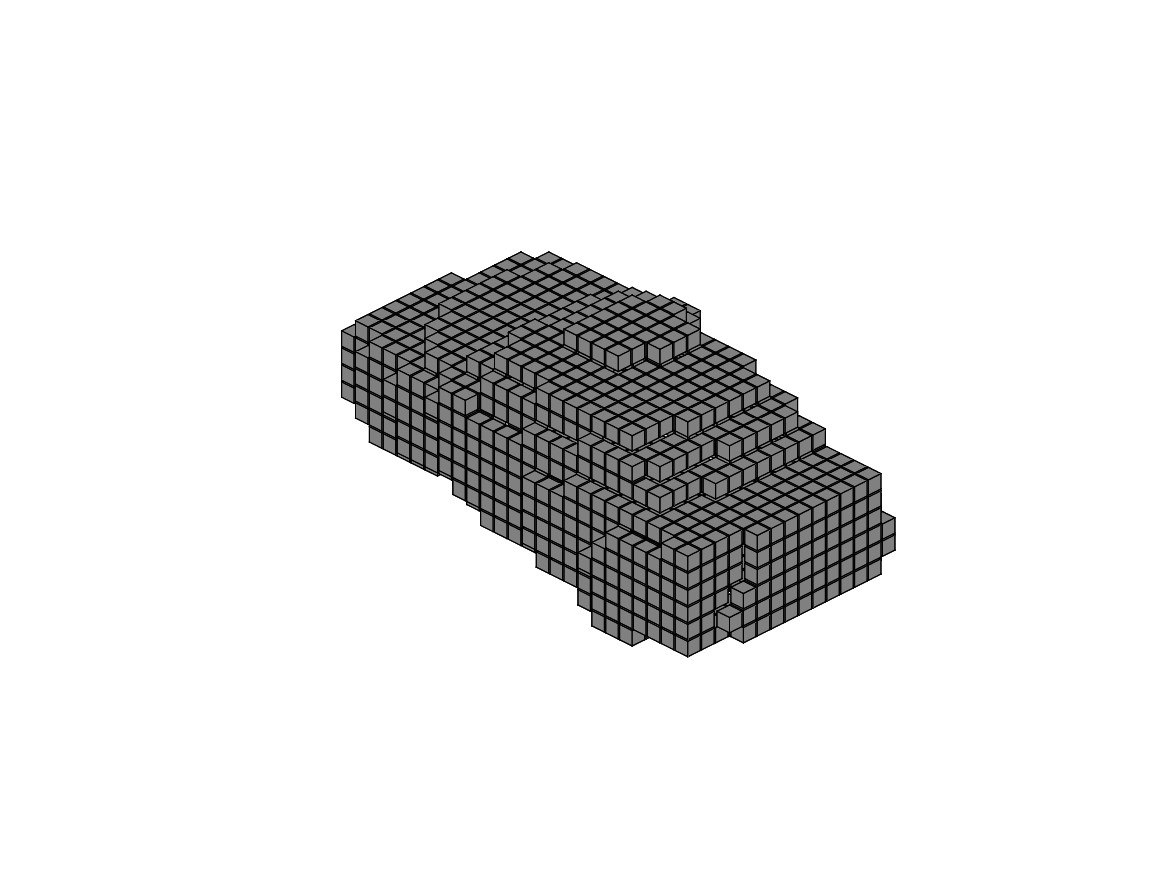
\includegraphics[width=3cm,trim={2cm 1cm 2cm 1cm},clip]{data/shapenet/hard/6_target_45}
  \end{subfigure}\\
  \begin{subfigure}[t]{0.425\textwidth}
    \vspace{0px}
    \includegraphics[width=6cm]{data/3d/hard/data_0_0}\\
    \hspace*{-0.25cm}\includegraphics[width=6.5cm]{data/3d/easy/colorbar_0}
  \end{subfigure}
  \begin{subfigure}[t]{0.2\textwidth}
    \vspace{0px}
    \includegraphics[width=3cm,trim={2cm 1cm 2cm 1cm},clip]{data/3d/hard/0_input_45}
  \end{subfigure}
  \begin{subfigure}[t]{0.2\textwidth}
    \vspace{0px}
    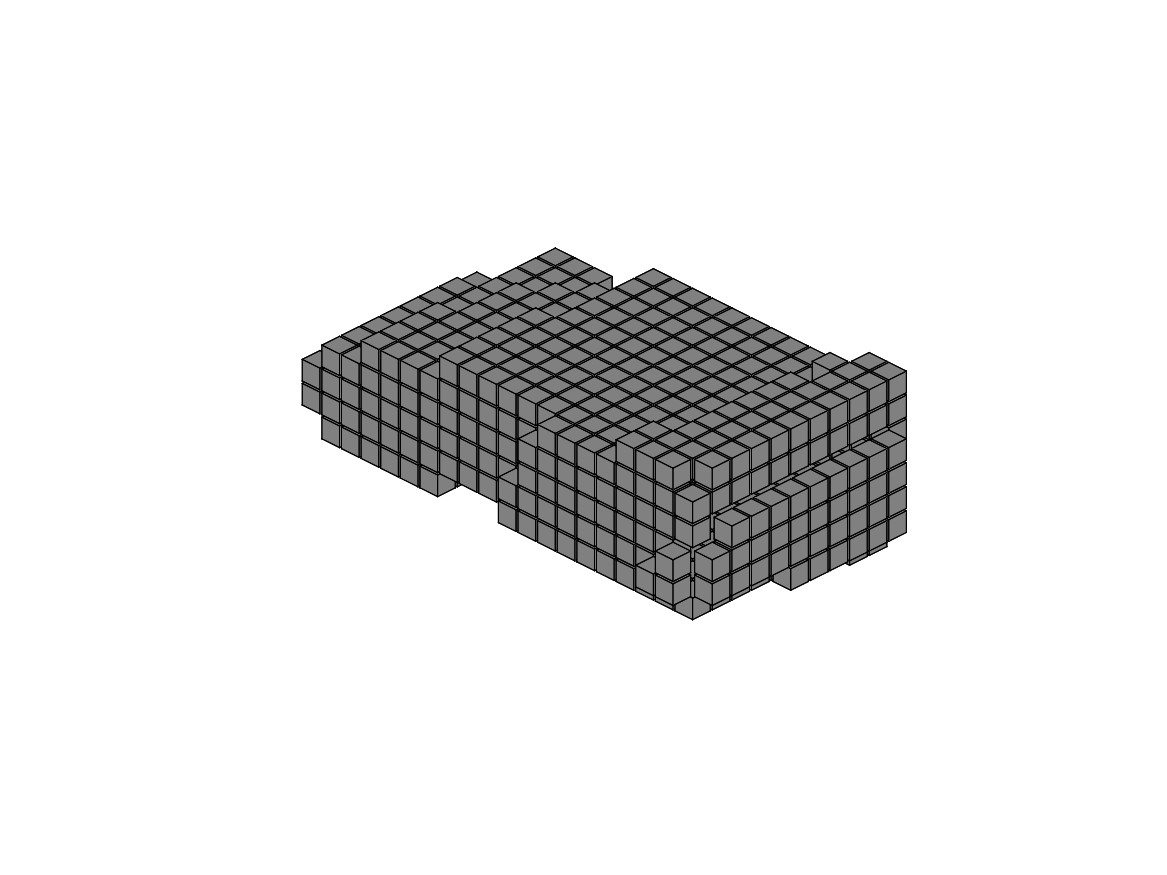
\includegraphics[width=3cm,trim={2cm 1cm 2cm 1cm},clip]{data/3d/hard/0_target_45}
  \end{subfigure}
  \vskip 6px
  % TODO short caption
  % TODO text
  \caption{Examples from the created datasets corresponding to a model from ShapeNet
  (top) and a cuboid (bottom). In both cases we show heights $8 + 2i$ for $0 \leq i < 8$,
  \ie horizontal slices, illustrating the
  observed points, the computed partial free space and the ground truth shape.
  Additionally, we show 3D visualizations of the observed points and the corresponding
  shape; both in voxelized form.}
  \label{fig:data-3d-examples}
\end{figure}

% TODO artifacts
Figure \ref{fig:data-simplification} illustrates the variety of car models covered.
In addition, the simplified meshes are shown; we want to note that
some meshes, \eg from the Humvee on the right, are quite complex and this
complexity is vastly reduced during simplification. However, this also
incurs some loss of detail which we accept as voxelization is performed in
low resolution anyway. Figure \ref{fig:data-3d-examples} shows the corresponding voxelizations
for both ShapeNet and the 3D cuboids dataset when using
$\lambda_{\text{hit}} = 50$, $\theta_{\text{ignore}} = 0.1$, and
$2u \times 2v = 24 \times 32$ as resolution for the depth image. The noise
can best be observed in the horizontal slices of the sown volumes
-- especially considering the ignored rays.
More examples can be found in Appendix~\ref{ch:appendix-data}.

\section{KITTI}
\label{sec:data-kitti}

% TODO real bounding boxes
%\begin{figure}
%  \centering
%  \begin{tikzpicture}
    
    % https://tex.stackexchange.com/questions/40840/put-a-node-behind-another-in-a-tikz-diagram
%    \begin{scope}[on background layer]
%      \node at (0, 0) {
%        \includegraphics[height=5cm]{data/kitti/snapshot_00_rect}
%      };
%    \end{scope}
    
%    \node[rectangle,minimum width=3cm,minimum height=1cm,draw=red!75] (rect) at (-2.5,-0.25){};
%    \node[rectangle,draw=red!75] (excerpt) at (-4, 2.5) {
%      \includegraphics[height=3cm]{data/kitti/snapshot_01_rect}
%    };
    
%    \draw[-,red!75] (rect.north west) -- (excerpt.south west);
%    \draw[-,red!75] (rect.north east) -- (excerpt.south east);
%  \end{tikzpicture}
%  \vskip 6px
  % TODO short caption
%  \caption{Illustration of the raw point cloud extracted from the first
%  city drive in KITTI,
%  \ie \lstinline!2011_09_26_drive_0001!. The provided 3D bounding box corners are
%  marked green and points within a bounding box are marked blue. The top image
%  shows the scene from bird's eye view.}
%  \label{fig:data-kitti}
%\end{figure}

% TODO image of point cloud with bounding boxes
The KITTI dataset
is a standard dataset and benchmark for a variety of computer vision tasks.
Beneath stereo image pairs, point clouds were captured from a moving vehicle
using a $360^\circ$ Velodyne LiDAR sensor\footnote{
  Details can be found in \cite{GeigerLenzUrtasun:2012} as well as in the corresponding
  manual at \url{http://www.velodynelidar.com/lidar/products/manual/HDL-64E\%20Manual.pdf0}.
}. An example of a captured point cloud is shown in Figure \ref{fig:introduction}.
Annotations
include -- among others -- 3D bounding boxes for all cars visible
on the image plane (\ie point clouds were not annotated in $360^\circ$).
As discussed in Chapter \ref{ch:problem}, we tackle shape completion of
an individual object. Therefore, we assume a 3D object detector to be given.
Due to the limited scope of this thesis, we use the provided ground truth 3D
bounding boxes for our experiments. These are first extracted, scaled and
the corresponding points are voxelized. Free space is then computed using
ray tracing.
%Both is discussed in detail in the following.

%\subsection{3D Bounding Boxes}
% TODO avoid e_bb if not needed.
% TODO character for extents/dimensions!
%The point cloud is provided relative to the sensor's center; the corresponding
%3D bounding boxes are specified by defining the translation of its center
%$t_{\text{bb}}$, the rotational angle around the vertical (height) axis expressed in
%terms of the derived rotation matrix $\mathcal{R}_{\text{bb}}$, and the
%dimensions, \ie extents, of the box $e_{\text{bb}}$
%in terms of width $e_{\text{bb},1}$, height $e_{\text{bb},2}$ and depth
%$e_{\text{bb},3}$.

\subsection{Point Cloud Voxelization}

Each ground truth 3D bounding box is provided in the form of its center,
\ie translation from the sensor's center, the extents in terms of width,
height and depth as well as the rotational angle along the (vertical)
height axis. For voxelization, the bounding boxes are rotated
to be axis aligned and then scaled to the unit cube, \ie $[0,1]^3$.
Again, we make sure to scale all axes equally such that the
observations do not get skewed.

\subsection{Free Space Voxelization}

To voxelize free space, we follow the same approach as before, \ie ray tracing.
Again, we consider partial free space as the Velodyne sensor has difficulties with
reflective and transparent surfaces. In particular we found that many
rays go through the annotated cars and hit points in the background. 
Considering partial free space, this effect is reduced by only tracing
rays that correspond to points within the 3D bounding box.
We then compute ray-box intersections between all rays and all voxels
using the same subdivision into voxels as used before to avoid errors.
Still, some points are prone to lie within the observed car -- \eg at the
height of the windows -- causing voxels to erroneously be labeled as
free space.

\subsection{Filtering}

\begin{figure}
  \centering  
  \vspace{-0.25cm}
  \begin{subfigure}[t]{0.425\textwidth}
    \vspace{0px}
    \includegraphics[width=6cm]{data/kitti/150_1500_30_3/data_0_0}\\
    \hspace*{-0.25cm}\includegraphics[width=6.5cm]{data/kitti/150_1500_30_3/colorbar_0}
  \end{subfigure}
  \begin{subfigure}[t]{0.2\textwidth}
    \vspace{0px}
    \includegraphics[width=3cm,trim={2cm 1cm 2cm 1cm},clip]{data/kitti/150_1500_30_3/0_input_45}
  \end{subfigure}
  \begin{subfigure}[t]{0.2\textwidth}
    \vspace{0px}
    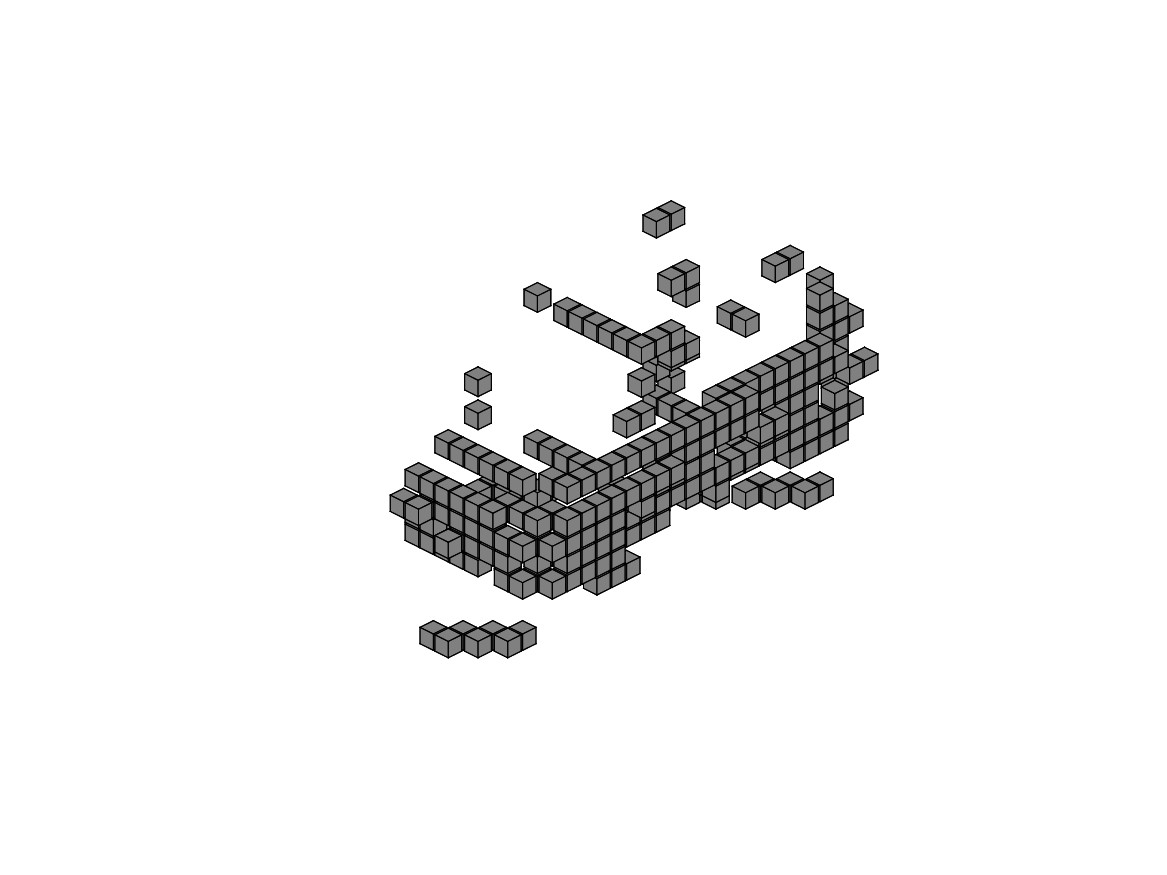
\includegraphics[width=3cm,trim={2cm 1cm 2cm 1cm},clip]{data/kitti/150_1500_30_3/0_input_135}
  \end{subfigure}\\[-4px]
  \begin{subfigure}[t]{0.425\textwidth}
    \vspace{0px}
    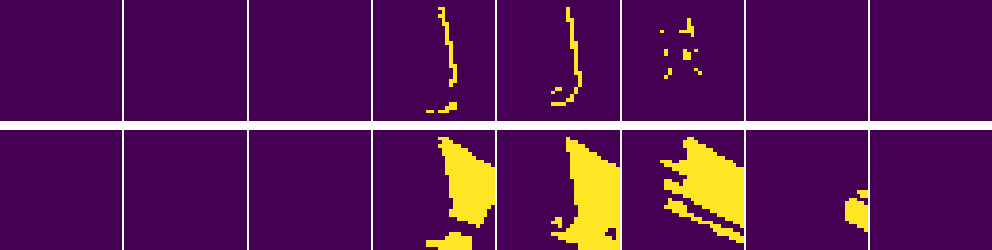
\includegraphics[width=6cm]{data/kitti/150_1500_30_3/data_1_0}\\
    \hspace*{-0.25cm}\includegraphics[width=6.5cm]{data/kitti/150_1500_30_3/colorbar_0}
  \end{subfigure}
  \begin{subfigure}[t]{0.2\textwidth}
    \vspace{0px}
    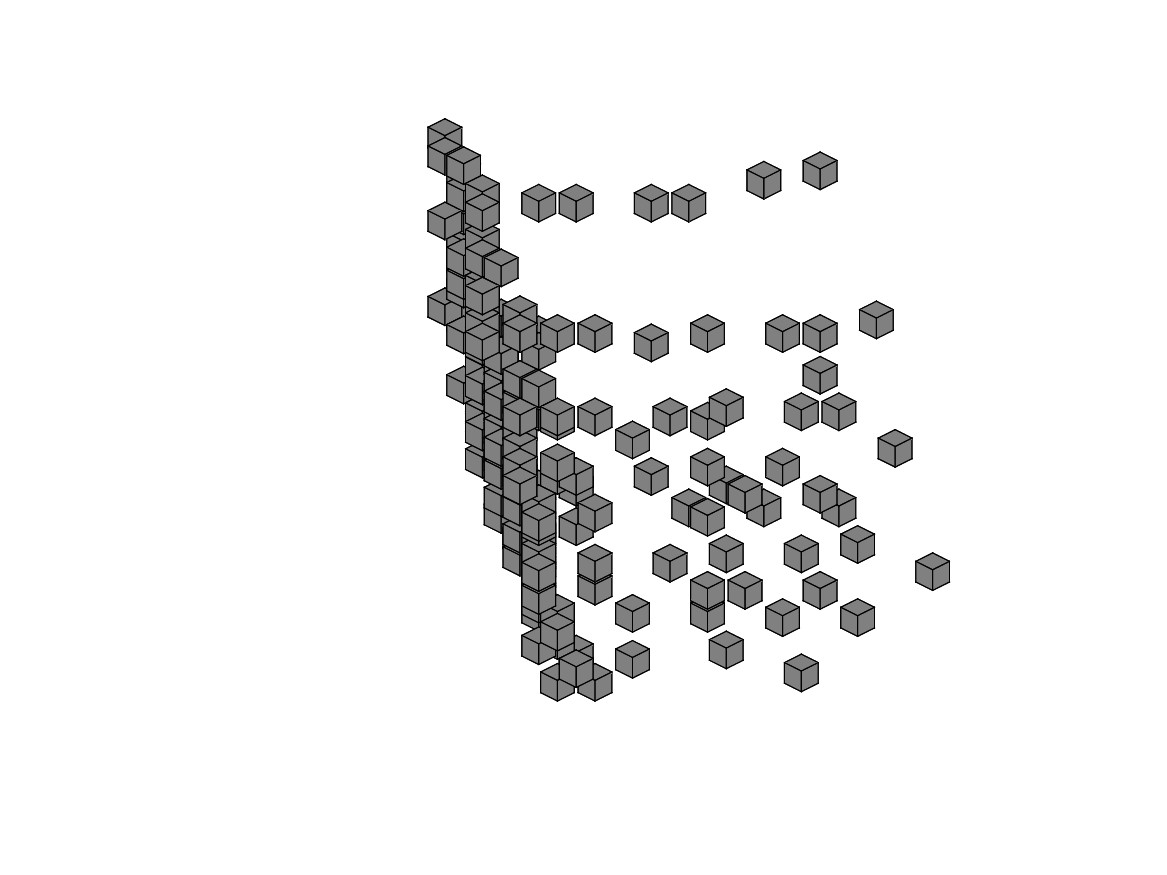
\includegraphics[width=3cm,trim={2cm 1cm 2cm 1cm},clip]{data/kitti/150_1500_30_3/1_input_45}
  \end{subfigure}
  \begin{subfigure}[t]{0.2\textwidth}
    \vspace{0px}
    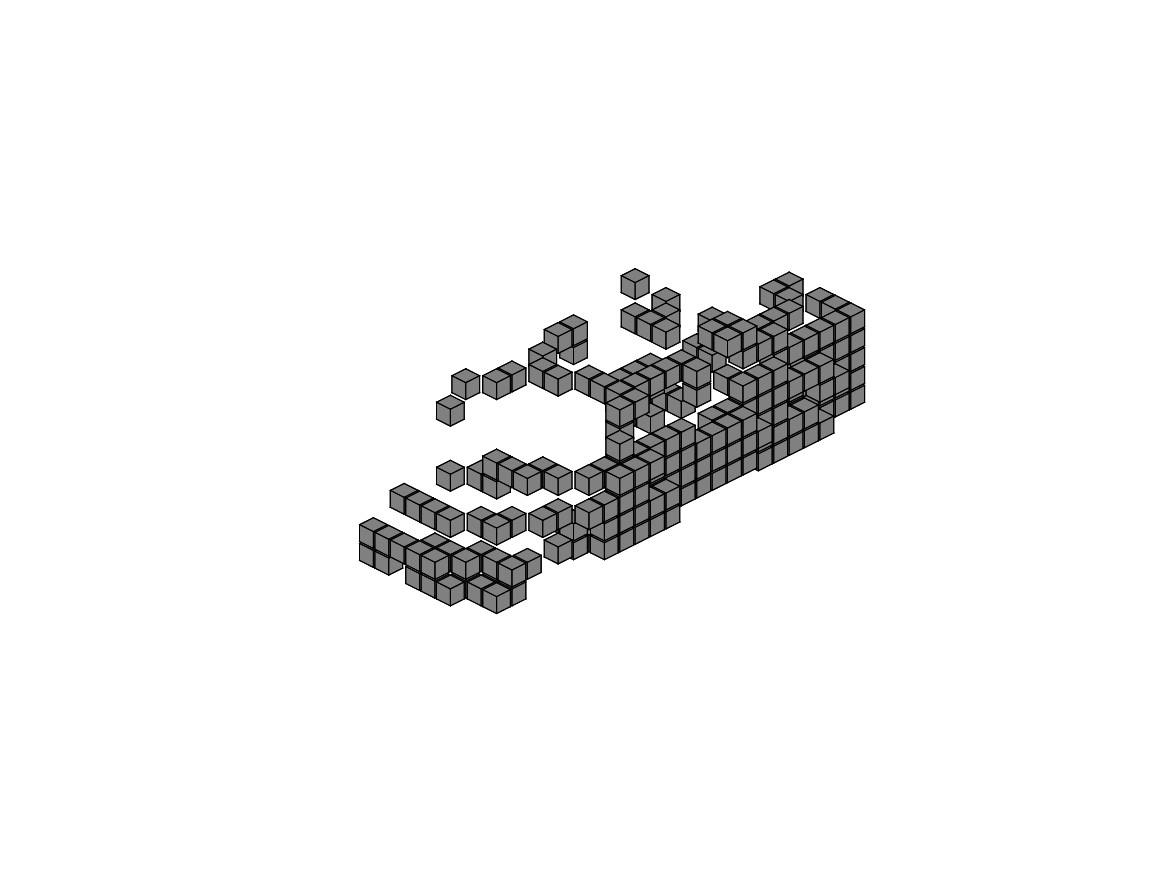
\includegraphics[width=3cm,trim={2cm 1cm 2cm 1cm},clip]{data/kitti/150_1500_30_3/1_input_135}
  \end{subfigure}
  
  % TODO short caption
  % TODO text
  \caption{Two examples as extracted from KITTI. Again, we show horizontal slices
  of the voxelized points and the corresponding free space together with 3D visualizations
  of the observed points and the corresponding shape.}
  \label{fig:data-kitti-examples}
\end{figure}

Using all the voxelized observations to learn shape completion is not
realistic within the scope of this thesis -- especially as many
observations contain only very few observed points and erroneous free space.
Therefore, we filtered the voxelized observations to obtain an easier
dataset. First, we require that at least
$n_{1,\min}$ points are observed and $n_{0, \min}$ voxels correspond
to free space:
\begin{align}
  \sum_{i = 1}^R \mathds{1}[x_i = 1] \overset{!}{>} n_{1,\min}\quad\text{ and }\quad\sum_{i = 1}^R \mathds{1}[x_i = 0] \overset{!}{>} n_{0,\min};
\end{align}
Second, we require the distance of the 3D bounding
box to the Velodyne sensor to be less than $t_{\max}$. In practice, the
three constraints ensure that the extracted dataset is manageable to tackle
in the course of this thesis. Higher difficulties can then
be obtained by lowering $n_{1,\min}$ and $n_{0,\min}$ and increasing $t_{\max}$,
respectively. The exact constraints and some statistics are provided in
Chapter \ref{ch:experiments} when conducting experiments on KITTI.

\subsection{Discussion}

Overall, it is fair to say that KITTI's Velodyne data exhibits several
distinct noise patterns -- that we also tried to model in our synthetic datasets.
The examples chosen in Figure \ref{fig:data-kitti-examples} were manually selected to
illustrate that some bounding boxes clearly depict cars. Still, even in this example,
we notice some artifacts. For example, due to noise and discretization, observed
points frequently lie inside the car. This is problematic as the corresponding
free space derived by ray tracing is partly invalid. We also notice that this 
happens more frequently at the height of the car's windows -- 
sometimes the Velodyne's rays hit other objects inside the
car instead, \eg seats. In Appendix \ref{ch:appendix-data}, we show further
examples.
